\documentclass[11pt]{beamer}

% Opciones adicionales

\usepackage[utf8]{inputenc}
\usepackage[spanish]{babel}
\usepackage{amsmath}
\usepackage{amsfonts}
\usepackage{amssymb}
\usepackage{graphicx}
\usepackage{lipsum}
\usepackage{ragged2e}
\usepackage{hyperref}
\usepackage{float}
\usepackage{url}


\usepackage[backend=biber,style=authoryear,doi=false,isbn=false,url=false,eprint=false]{biblatex}
\addbibresource{bibliografia.bib}



% Configurar el tamaño de las notas a pie de página
\renewcommand{\footnotesize}{\tiny}

% Definir comando para referencia en el pie de página
\newcommand{\footreferencia}[1]{\footnote{\fullcite{#1}}}

% Información del título
\title{“Distribuciones de probabilidad en la Florescencia Resonante Intermitente”}

\author[Kevin Martínez Franco]
{Lic. Kevin Martínez Franco }

\institute[CIICAP]{
	\inst{1}
		Universidad Autónoma del Estado de Morelos\\
		\vspace{2mm}
	\inst{2}
            Instituto De Investigación En Ciencias Básicas y Aplicadas
		 
}
\date{\today}
\subtitle{Métodos Matemáticos Avanzados }

\AtBeginSection[]
{
	\begin{frame}<beamer>{Contenido}
		\tableofcontents[currentsection,currentsubsection]
	\end{frame}
}

\begin{document}

        \begin{frame}
		\maketitle
	\end{frame}


        \begin{frame}{Contenido}
		\tableofcontents
	\end{frame} 


	\section{Planteamiento del problema}
 \begin{frame}{Sistemas Cuánticos Abiertos}

\justifying


\begin{itemize}
    \item Un \textbf{sistema cuántico abierto} es un sistema cuántico que interactúa con un entorno externo, lo que provoca que su dinámica no esté completamente aislada.
    \item A diferencia de los sistemas cerrados, donde la evolución es unitaria y conservativa, los sistemas abiertos \textbf{pierden coherencia} y pueden intercambiar energía o partículas con el entorno.
\end{itemize}

\vspace{0.5em}
\textbf{Características de los Sistemas Cuánticos Abiertos}

\begin{itemize}
    \item La interacción con el entorno genera \textbf{decoherencia} y \textbf{disipación}, lo que afecta las propiedades cuánticas del sistema.
    \item El estado del sistema ya no se describe solo por una función de onda pura, sino por un \textbf{operador de densidad} que representa probabilidades de diferentes estados.
    \item La evolución de estos sistemas se modela mediante la \textbf{ecuación maestra de Lindblad} y con \textbf{Trayectorias cuánticas}.
\end{itemize}


\end{frame}


    \begin{frame}{Planteamiento del problema}
        \justifying
        Abordamos el fenómeno de fluorescencia resonante intermitente, que describe la alternancia aleatoria entre per\'iodos de emisión frecuente de fotones ("brillantes") y periodos de nula emisión ("oscuros") en un átomo excitado por un láser \footfullcite{PlKn}. 
        
        Consideramos un átomo de tres niveles interactuando con un láser que excita la transici\'on 
        $|e \rangle - |g \rangle$ con frecuencia de Rabi $\Omega$, y que decae a raz\'on $\gamma$, generando un per\'iodo brillante. 
        El estado $|e \rangle$ decae ocasionalmente a raz\'on $\gamma_d$ a un estado metaestable $|a \rangle$ que interrumpe la fluorescencia en $|e \rangle - |g \rangle$. Al decaer el estado $|a \rangle$ a $|g \rangle$ a raz\'on $\gamma_a$ vuelve la fluorescencia. Las razones de emisi\'on espont\'anea cumplen 
        $\gamma \gg \gamma_d,\gamma_a$.
        
        
    \end{frame}
    
    \begin{frame}{El sistema}
        \justifying
        Para simular este proceso, utilizamos el método de Trayectorias Cuánticas \footfullcite{Carmichael}, que modela la dinámica de emisión fotónica del sistema. 
        \begin{center}
           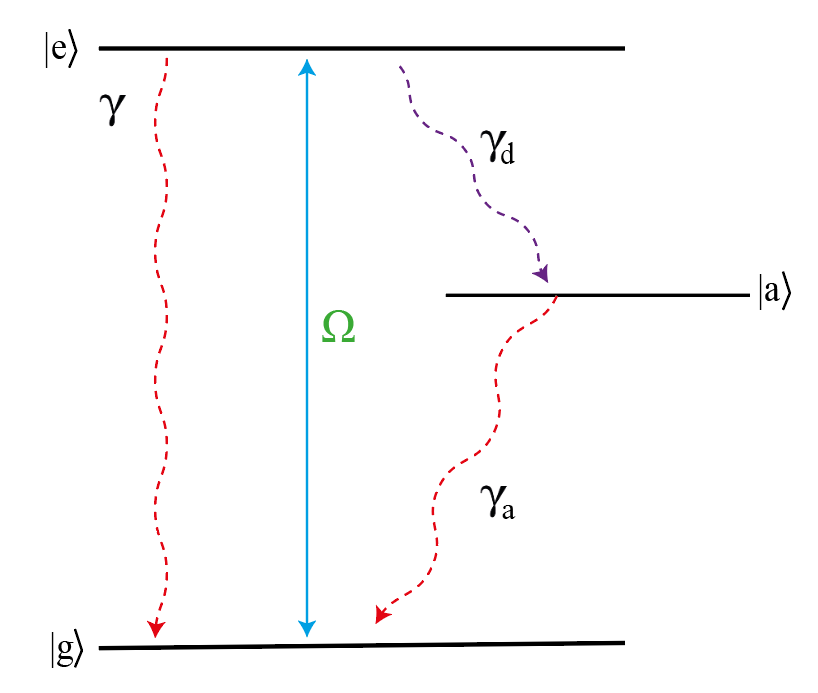
\includegraphics[width=0.65\linewidth]{1 sistema.png} 
        \end{center}
        \end{frame}


    
    \section{Trayectorias Cuánticas}
    \begin{frame}{Trayectorias Cuánticas}

     
        Para simular una trayectoria cu\'antica de saltos resolvemos la ecuaci\'on de Schr\"odinger $i\hbar \dot{|\Psi \rangle} =H_{\mathrm{eff}} |\Psi \rangle$, donde \\
        \begin{center}
            $H_{\mathrm{eff}} = H - i \frac{\gamma}{2} A_{ee} -i \frac{\gamma_d}{2} A_{ee} - i \frac{\gamma_a}{2} A_{aa}$ 
        \end{center}
        
        \\
        es un Hamiltoniano efectivo no-Hermitiano, $H = \Delta A_{eg} A_{ge} + \frac{\Omega}{2} (A_{eg} + A_{ge})$ es el Hamiltoniano de la interacci\'on \'atomo-l\'aser, y los siguientes t\'erminos denotan emisi\'on espont\'anea. 
    \end{frame}
    
    
    
    
    \begin{frame}
        \justifying
        Una trayectoria consiste en intervalos de evoluci\'on no unitaria hasta que se emite un fot\'on en alguna de las transiciones con 
        probabilidad $p_k(t) = \delta t \langle \Psi_c(t) | \mathcal{C}_k^\dagger \mathcal{C}_k | \Psi_c(t) \rangle$, 
        donde $\mathcal{C}_k = \sqrt{\gamma_k} A_{kk}$ son los operadores de colapso que representan los diferentes canales de emisión. De no emitirse un fot\'on el sistema contin\'ua siguiendo la ecuaci\'on de Schr\"odinger.
        
        El promedio en el ensamble de muchas trayectorias reproduce la evolución del operador de densidad $\rho$, que obedece la ecuación maestra $\dot{\rho} = -\frac{i}{\hbar} [H, \rho] + \mathcal{L}_D \rho$, donde $\mathcal{L}_D$ es el superoperador de Lindblad, que modela las emisiones espontáneas entre los diferentes niveles atómicos. 
    \end{frame}

   

    \begin{frame}{Algoritmo de Saltos Cuánticos de Carmichael}
        \justifying
        \vspace{0.3cm}
    
        \begin{enumerate}
            \item \textbf{Inicialización}: El sistema comienza en un estado puro inicial $\ket{\psi(0)}$.
            \item \textbf{Evolución Continua}: Se resuelve la ecuación de Schrödinger no hermítica:
            \[
            \frac{d}{dt}\ket{\psi(t)} = -\frac{i}{\hbar} H_{\text{eff}} \ket{\psi(t)}
            \]
            donde $H_{\text{eff}} = H - \frac{i}{2} \sum_j \gamma_j C_j^\dagger C_j$.
            
            \item \textbf{Detección de Saltos}: La probabilidad de salto en cada $\delta t$ se compara con un número aleatorio.
            
            \item \textbf{Salto Cuántico}: Si ocurre un salto, el estado colapsa a través de un operador $C_j$, y se normaliza:
            \[
            \ket{\psi(t)} \rightarrow \frac{C_j \ket{\psi(t)}}{\sqrt{\langle \psi(t) | C_j^\dagger C_j | \psi(t) \rangle}}.
            \]
            
            \item \textbf{Repetición}: Se repiten los pasos 2-4 hasta completar el tiempo de evolución.
        \end{enumerate}
    
    
    
        \vspace{0.2cm}
        \footnotesize
        \footfullcite{Carmichael}
    \end{frame}
    \section{Simulaciones}
    

    
    
    
    \begin{frame}{Simulación de las trayectorias. }
        \justifying
        En la Fig.~2, mostramos un fragmento de una trayectoria t\'ipica, mostrando per\'iodos brillantes con oscilaciones de Rabi, y per\'iodos oscuros. A la derecha Mostramos el promedio en un ensamble de 4000 trayectorias, el cual se compara muy bien con el resultado obtenido con la ecuaci\'on maestra. Par\'ametros: $\Omega=3.5\gamma$, $\Delta=0$, $\gamma_d=0.95\gamma$, $\gamma_d=0.05\gamma$, $\gamma_a =0.015 \gamma$. 
    
        
        \begin{center}
        
\includegraphics[width=1.1\linewidth]{Presentacion MMA/zoom y meq vs tj.png} 
        \end{center}
        

        
    \end{frame}

\begin{frame}
    
        \textbf{Ecuación Maestra vs. Trayectorias Cuánticas}
        
        \begin{itemize}
            \item La \textbf{Ecuación Maestra} describe la evolución temporal promedio del estado del sistema cuántico, considerando todas las posibles interacciones con el entorno.
            \item Las \textbf{Trayectorias Cuánticas} (también conocidas como métodos de Monte Carlo cuántico) simulan la evolución de estados individuales del sistema, incluyendo saltos cuánticos aleatorios.
        \end{itemize}
        
        \textbf{Resultados Experimentales Consistentes}
        
        \begin{itemize}
            \item Ambos enfoques, aunque diferentes en su formulación, \textbf{predicen los mismos resultados experimentales} en términos de poblaciones y observables medibles.
            \item La equivalencia se debe a que las trayectorias cuánticas, al promediarse sobre muchas realizaciones, \textbf{reproducen la dinámica promedio} descrita por la ecuación maestra.
        \end{itemize}
        
      
        
    
          Esto demuestra que las trayectorias cuánticas son una herramienta válida y precisa para simular sistemas cuánticos abiertos, ofreciendo además \textbf{intuición sobre procesos individuales} como saltos cuánticos y tiempos de espera.
        
       
    
    \end{frame}

\begin{frame}{Algoritmo para Calcular Períodos Oscuros}
    
    \textbf{Descripción Simplificada del Algoritmo}
    
    \begin{enumerate} \item \textbf{Registro de Eventos de Colapso} \begin{itemize} \item Durante la simulación, se registran eventos de colapso en ciertos tiempos. \item Cada colapso corresponde a una transición específica en el sistema. \end{itemize} \vspace{0.5em} \item \textbf{Identificación de Períodos} \begin{itemize} \item \textbf{Períodos Brillantes}: Intervalos donde el sistema emite fluorescencia. \item \textbf{Períodos Oscuros}: Intervalos donde no hay emisión de fluorescencia. \end{itemize} \vspace{0.5em} \item \textbf{Detección de Transiciones Clave} \begin{itemize} \item Se enfocan en colapsos específicos que marcan el inicio y fin de los períodos. \item Por ejemplo, un colapso de tipo 1 indica el inicio de un período brillante. \end{itemize} \vspace{0.5em} \item \textbf{Cálculo de Duraciones} \begin{itemize} \item \textbf{Períodos Brillantes}: Duración = tiempo de fin - tiempo de inicio. \item \textbf{Períodos Oscuros}: Duración = inicio del siguiente período brillante - fin del período brillante actual. \end{itemize} \vspace{0.5em} \item \textbf{Almacenamiento y Análisis} \begin{itemize} \item Se guardan las duraciones para análisis estadístico. \item Permite calcular tiempos promedio y visualizar patrones de intermitencia. \end{itemize} \end{enumerate}
    
\end{frame}

\begin{frame}
\justifying
El procedimiento de c\'alculo de trayectorias permite recoger la informaci\'on de fotoemisiones y estad\'istica de los per\'iodos brillantes y oscuros. Esto se logra mejor si hacemos una trayectoria muy larga en lugar de muchas trayectorias cortas. Se pueden obtener las distribuciones de las duraciones de los periodos oscuros y brillantes, que siguen distribuciones exponenciales: 
$$ P_O = \frac{1}{T_O} e^{-t/T_O}, \qquad  
    P_B = \frac{1}{T_B} e^{-t/T_B} ,$$
con duraciones promedio
$$ T_O = \gamma_a^{-1}, \qquad T_B = \frac{2\Omega^2 + \gamma^2 + 4\Delta^2}{\gamma_d \Omega^2} .$$

\end{frame}
\begin{frame}
La figura 3 muestra las duraciones de los per\'iodos oscuros y su distribuci\'on obtenidas de una trayectoria larga de duraci\'on $\gamma t = 10^6$. 

\vspace{-0.2em}
\begin{center}
	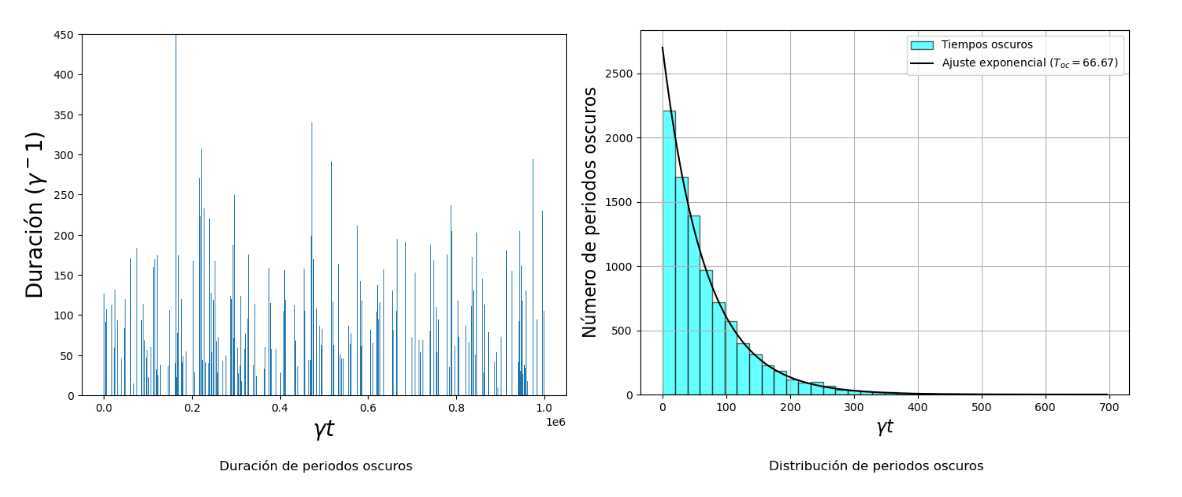
\includegraphics[width=1.1\linewidth]{5 dist dur.png}
\end{center}
\end{frame}

\begin{frame}{Distribución de Poisson en Mecánica Cuántica y Períodos Oscuros}

\textbf{Distribución de Poisson}

\begin{itemize}
    \item La distribución de Poisson describe la probabilidad de que ocurra un número determinado de eventos en un intervalo de tiempo fijo, cuando los eventos son independientes y ocurren a una tasa promedio constante.
    \item Matemáticamente, se expresa como:
    \[
    P(n; \lambda) = \frac{\lambda^n e^{-\lambda}}{n!}
    \]
    donde \( \lambda \) es el número promedio de eventos en el intervalo.
\end{itemize}
\end{frame}

\begin{frame}{Distribución de Poisson en Óptica Cuántica y Períodos Oscuros}
\textbf{Uso en Óptica Cuántica}
\begin{itemize}
    \item En óptica cuántica, la distribución de Poisson aparece en procesos de emisión espontánea y detección de fotones, donde el número de emisiones o detecciones en un intervalo de tiempo sigue esta distribución.
    \item Es fundamental en la teoría de fotones y en experimentos de fluorescencia resonante, donde los períodos de emisión de fotones (brillantes) y los períodos oscuros pueden analizarse estadísticamente.
\end{itemize}
\end{frame}

\begin{frame}
\textbf{Períodos Oscuros y Distribución de Poisson}

\begin{itemize}
    \item Que los períodos oscuros sigan una distribución de Poisson implica que los eventos de emisión están separados por intervalos de no emisión (oscuros) que son estadísticamente independientes.
    \item Esta independencia sugiere que el sistema tiene una "memoria" limitada y que, después de un período oscuro, el sistema no "recuerda" cuándo ocurrió el último evento, cumpliendo así el principio de Markov.
\end{itemize}

\end{frame}
\begin{frame}
\textbf{Implicaciones}

\begin{itemize}
    \item La aparición de una distribución de Poisson en los períodos oscuros es clave para entender la dinámica del sistema y su naturaleza cuántica, indicando que los eventos de emisión y no emisión pueden modelarse como procesos estocásticos, independientes y con una tasa de ocurrencia constante.
\end{itemize}

\end{frame}




\begin{frame}{Distribución de tiempos de espera en un Sistema de Dos Niveles con Diferentes Frecuencias de Rabi}



     La figura muestra la distribución de la emisión en un sistema de dos niveles bajo la influencia de campos con diferentes frecuencias de Rabi.
    Se consideran dos casos:

        \textbf{Frecuencia de Rabi \(\Omega = 1\)}: Representa un campo de intensidad moderada. \\
       \textbf{Frecuencia de Rabi \(\Omega = 3\)}: Representa un campo más intenso.

  
\begin{figure}
    \centering
    
\includegraphics[width=0.9\linewidth]{Presentacion MMA/2LA.png}
   
    \label{fig:enter-label}
\end{figure}

\end{frame}
\begin{frame}
\textbf{Observaciones Clave}


\begin{itemize}
    \item \textbf{Para \(\Omega = 1\)}:
    \begin{itemize}
        \item El sistema exhibe una distribución de emisión característica, posiblemente con períodos más largos entre eventos de emisión.
        \item La probabilidad de transición es menor debido a la menor intensidad del campo.
    \end{itemize}
    \item \textbf{Para \(\Omega = 3\)}:
    \begin{itemize}
        \item La distribución muestra una mayor tasa de emisión, indicando transiciones más frecuentes entre los niveles.
        \item El campo más intenso aumenta la probabilidad de transición, afectando la dinámica del sistema.
    \end{itemize}
\end{itemize}
\end{frame}

\begin{frame}{Combinación de Distribuciones en un Sistema de Tres Niveles con Shelving}

\textbf{Mezcla de Distribuciones Independientes}

\begin{itemize}
  

    \item La dinámica del sistema implica:
    \begin{itemize}
        \item Transiciones entre \( |g\rangle \) y \( |e\rangle \) — comportamiento de un sistema de \textbf{dos niveles}
        \item Transiciones hacia y desde \( |m\rangle \) — introducen \textbf{períodos oscuros} (no emisión de fotones)
    \end{itemize}
    \vspace{0.5em}
    \item Las \textbf{distribuciones de tiempos de espera} del sistema de dos niveles y los \textbf{tiempos oscuros} asociados al estado metastable se \textbf{combinan de forma independiente} en la distribución total
\end{itemize}
\end{frame}

\begin{frame}
\textbf{Influencia de la Tasa de Decaimiento al Estado Metastable}

\begin{itemize}
    \item La \textbf{tasa de decaimiento} del estado excitado al estado metastable (\( \gamma_{em} \)):
    \begin{itemize}
        \item Determina la \textbf{frecuencia con la que el sistema entra en el estado metastable}
        \item Afecta el \textbf{número de períodos oscuros} en la distribución final
    \end{itemize}
    \vspace{0.5em}
    \item Una \textbf{tasa de decaimiento mayor} implica:
    \begin{itemize}
        \item \textbf{Más períodos oscuros} 
        \item Alteración en la distribución total de tiempos de espera
    \end{itemize}
\end{itemize}

\textbf{Conclusión}

\begin{itemize}
    \item En el sistema de tres niveles con \textit{shelving}:
    \begin{itemize}
        \item Las distribuciones de tiempos de espera del sistema de dos niveles y los tiempos oscuros se \textbf{superponen} para formar la distribución total
        \item La \textbf{tasa de decaimiento al estado metastable} es clave para determinar la \textbf{estructura de la distribución} de los tiempos de emisión y espera
    \end{itemize}
\end{itemize}
\end{frame}


\begin{frame}{Distribución de tiempos de espera 3LA con frecuencia de $\Omega = 1$}
\begin{figure}
    \centering
    
\includegraphics[width=1\linewidth]{Presentacion MMA/3LA .png}

    \label{fig:enter-label}
\end{figure}
\end{frame}

\begin{frame}{Distribución de tiempos de espera 3LA con frecuencia de $\Omega = 3.5$}
\begin{figure}
    \centering
    
\includegraphics[width=1\linewidth]{Presentacion MMA/3lafuerte.png}

    \label{fig:enter-label}
\end{figure}
\end{frame}

\begin{frame}{Distribución de Tiempos de Espera en Óptica Cuántica}

\textbf{Distribución de Tiempos de Espera}

\begin{itemize}
    \item En sistemas cuánticos, los tiempos de espera representan los intervalos entre eventos de emisión (por ejemplo, detección de fotones).
    \item La distribución de estos tiempos de espera también puede seguir una distribución de Poisson, pero en términos de tiempo continuo, conocida como una distribución exponencial:
    \[
    P(t) = \frac{1}{\tau} e^{-t/\tau}
    \]
    donde \( \tau \) es el tiempo promedio de espera entre eventos.
\end{itemize}
\end{frame}


\begin{frame}
\textbf{Períodos Oscuros y Tiempos de Espera}

\begin{itemize}
    \item Cuando se analizan los períodos oscuros, el tiempo de espera entre dos eventos de emisión puede describirse mediante una distribución exponencial.
    \item Esta relación implica que los eventos de emisión ocurren de manera aleatoria e independiente, lo cual es un indicio de la naturaleza estocástica del proceso.
\end{itemize}
\end{frame}
\begin{frame}
\textbf{Implicaciones}

\begin{itemize}
    \item La distribución exponencial de los tiempos de espera refuerza el principio de Markov, ya que la ocurrencia de cada evento no depende del tiempo que ha pasado desde el último.
    \item Esta propiedad es esencial en la mecánica cuántica, ya que permite modelar los eventos de emisión como un proceso de Poisson continuo en el tiempo.
\end{itemize}
\end{frame}

\begin{frame}{Conclusión}

\justifying
\begin{itemize}
    \item A lo largo de esta presentación, analizamos cómo las \textbf{distribuciones de probabilidad} describen los períodos brillantes y oscuros en la fluorescencia resonante intermitente de un sistema cuántico. Estas distribuciones permiten capturar la esencia estocástica de los procesos de emisión y no emisión en sistemas de dos y tres niveles.
    
  
    
    \item Este trabajo muestra cómo las herramientas de probabilidad y teoría de distribuciones aplicadas en mecánica cuántica proporcionan una representación precisa de la dinámica de emisión en sistemas de fluorescencia intermitente. Las distribuciones de probabilidad se presentan no solo como una descripción teórica, sino como una herramienta práctica para entender y predecir el comportamiento de sistemas cuánticos abiertos.
    
\end{itemize}

\end{frame}


\section{Bibliografia}
 \begin{frame}[allowframebreaks]
    \smaller
    \vspace{-0.4em}
    \printbibliography
\end{frame}

\end{document}